\chapter{Contribution}

As stated in previous section, IIDEAA is a set of newly developed tools that has not been used widely. It is crucial to test out IIDEAA thoroughly to detect possible bugs and identify current limitations of the framework so that we can improve. In this testing phase, we used projects from AxBench, a benchmark designed for Approximate Computing, to see whether both tools of IIDEAA can work properly. Additionally, since one of the ambitions for IIDEAA is to apply many Approximate Computing techniques to some Artificial Neural Network libraries, compatibility with these libraries is also an issue to address. The two library that were tested are DarkNet and Fast Artificial Neural Network(FANN). \\
~\\
The last objective of this internship is to create a new tool to generate Approximate variants based on the results of the 2 other tools. However, due the time constraint and delay of the internship because of visa issue, we have only started to work on and scratched the surface of this matter.\\

\section{Testing Environment}

It is worth to mention about the environment was used to conduct all tests with IIDEAA. In this framework, both Chimera and Bellerophon required LLVM-3.9.1, which was an older version of this compiler tools (current version is 7.0.0). Other than that, Bellerophon needs ParadisEO to be installed, because it uses the engine for Evolution Searching, as pointed out in the last chapter. Ideally, we would like to install everything in a separate machine for conveniences in testing, debug and modify the source code. However, installing LLVM was a difficult task and we ran into many problems. Luckily, The developer of the framework has provided us with the option of using a Docker image. This image was based on the ArchLinux default image and has everything needed for IIDEAA to run seemlessly.\\
\vspace*{3cm}

\section{Evaluating and Debugging IIDEAA}

\subsection{Applying IIDEAA to AxBench's benchmark}

AxBench is a benchmark containing a set of applications used for various approximate computing research. The benchmark was written in C++ and has some typical application from various domain such as finance, image processing, signal processing, etc. to investigate different aspects of Approximate Computing \cite{7755728}. The benchmark comes in with implemetations for both CPU and GPU. For the sake of simplicity, we've chosen to use CPU-based application to validate IIDEAA. \\
~\\
Aside from providing configuration files with desired parameter to Chimera and Bellerophon, in order to use the sample projects from AxBench with IIDEAA, some additions and modifications have to be made to these projects. First is the inclusion of CMake, a tool designed to build, test and package software, and its config file for each project. An important note when configuring the project using CMake is that generating a \textit{compile\_command.json} is necessary. This is due to the fact that both Chimera and Bellerophon will use it later on for syntax check and compilation. For Bellerophon case, some modifications needs to be made to make sure that the compiler has the correct path to the mutated files. \\
~\\
As mentioned in previous section, the user has to define how to calculate the error causes by precision loss and the reward gained from this loss to Bellerophon. Since the error metrics for each AxBench project was made public by the development team, we have used them to implement the error function. As for the reward function, it depends on how the Approximate Operator works. For this testing phase, we used two Operators implemeted by IIDEAA's developer, VPA and VPA\_Native. The two Operators are designed for Precision Scaling strategy as they modify the precision/data type. The reward function regarding to these two Operators will be discussed in the \textit{Result and Discussion} section. \\
~\\
In addition, source code modification sometimes is required to ensure that Bellerophon will have a function that can be called to execute the main part of the program, thus producing the approximated result for each variantions of the mutated program. Lastly, the user must also have a \textit{txt} file containing the result produced by the original version of the program. Because the source code of the program is the mutated one, it is more convenient to read the original result from the text file. Also, since the comparision between both version, original and mutated, is made for every variants, having the original source ran repeatedly is time consuming. \\
~\\
All the projects that were setup to be able to run by IIDEAA are available at: \url{https://github.com/nnkhoa/IIDEAA-Bench} \\

\subsection{Bugs encountered}

While testing IIDEAA with project from AxBench, we have found a few unwanted behaviors resided in the framework, the major ones being a few cases of incorrect mutation from Chimera caused by inaccurate interpretation of the source code's Abstract Syntax Tree. Another bug found was due to overlooking type casting in calculation while mutating, thus causing ambiguity when calling parameterized constructor as the object may not have constructor implemented for arguments in such data types. \\
~\\
To demonstrate bugs regarding the mutation process, consider the following example: 
\begin{minted}[fontsize=\normalsize]{cpp}
	#define DIV 1.5
	#define TEST(X, Y) (X + Y)
	
	int k, N;
	float r;			float x, y, z;
	
	/*
	 * initialize value for the variables
	 */
	
	r =   x/y; /*(1)*/	r = (float) k/N; /*(2)*/
	r = x/DIV; /*(3)*/	r = TEST(x, y) + z; /*(4)*/
\end{minted}
The correct behavior can be expected when mutating calculation (\textit{1}) is as follow:
\begin{minted}[fontsize=\normalsize]{cpp}
	r = (float) ::vpa::VPA(x, OP_1)/::vpa::VPA(y, OP_2);
\end{minted}
In general, the mutation process will travel down the Abstract Syntax Tree, searching for specific Tree Nodes that contain paticuliar symbols, depending on the definition of the Mutation Operator. For example, in the case of VPA\_Native Operator, Chimera will look for any Binary Operators or Binary Assign Operators such as add and subtract. Once these operators are found, Chimera will attempt to make modifications on the left hand side and/or right hand sign of the operator based on the API of the Approximate Operator. \\
~\\
From the above mutation, the \verb|VPA| constructor from the VPA\_Native approximate operator takes in 2 arguments. The first one is varible of either the following type: \textit{float}, \textit{double}, \textit{long double}. The second one contains the information about the precision to be changed when execute Bellerophon. \\
~\\
However, when mutate calculation (\textit{2}), while the mutation is correct as intended from the developers, it still causes error during compilation:
\begin{minted}[fontsize=\normalsize]{cpp}
	fatal error: call to constructor of ::vpa::VPA is ambiguous
	r = (float)((float) ::vpa::VPA(k, OP_1)/::vpa::VPA(N, OP_2));
						^
\end{minted}
To breifly explain, in (\textit{2}), the implicit cast was applied to make sure the result of the division \textit{k/N}, which is the division of 2 \textit{integer},is of the same type with \textit{r} (\textit{float}, in this case). However, Chimera does not consider the implicit cast and just mutates the calculation normally as if there was no cast. Thus, it will cause a "confusion" to the compiler as VPA\_Native does not have any constructor for integer variable. \\
~\\
In the case of (\textit{3}) and (\textit{4}), since \textit{DIV} and \textit{TEST} are macros, they does not count as either variable or function, and were not properly handled, thus causing errors as below when the mutation is complete:
\begin{minted}[fontsize=\normalsize]{cpp}
	// calculation number 3
	fatal error: expected ')'
        r =(float)( ::vpa_n::VPA(x , OP_0)/ DIV;
        									   ^
	note: to match this '('
        r =(float)( ::vpa_n::VPA(x , OP_0)/ DIV;
                        ^

	// calculation number 4
	fatal error: assigning to float from incompatible type vpa_n::VPA
        r =(float)( TEST(x, y) , OP_1) +::vpa_n::VPA( z, OP_1));
          ^~~~~~~~~~~~~~~~~~~~~~~~~~~~~~~~~~~~~~~~~~~~~~~~~~~~
\end{minted}
As can be seen, the mutation finished incorrectly as there are some missing syntaxes and parenthesis compare to the normal behavior. When we tried to extract and analyze information from the Abstract Syntax Tree of these calculations, fetching names of these macros, according to the position to the Binary Operator, returned empty, thus making the Mutator has nothing to base on and does not perform any mutation. However, the Abstract Syntax Tree still recognized that these are macros. This may be reason why the mutation process ended up being incorrect. \\
~\\
There are other undedired behaviors which led to program crashes, not due to the actual source code of the framework, but because of incompatability between project's dependencies and testing environment. For example, in the \textit{Sobel} project from AxBench, it is required that the system should have \textit{Boost Library} installed. However, compilation using the library was not sucessful due to version mismatch of a depedency named \textit{icu}, which is a core component of ArchLinux Docker image. Updating this component will require a full update of the current system. However, after the update, we experienced that this has interfered with the functionality of ParadisEO and inherently, Bellerophon, making them unusable. \\

\subsection{Analyzing and Debugging}

For the problems regarding Chimera, analyze and understand how the Abstract Syntax Tree works is the one way to approach these issues. With the problem of implicit cast with calculations that concern different data types, to avoid further problems like this in the future, we assume that the variables used in the calculation all have different data types to the casting type. Because of this, we make sure that if there are any implicit cast that is detected during the mutation process, we will mutate each varible, applying the implicit cast before further mutation. 
\begin{figure}[H]
%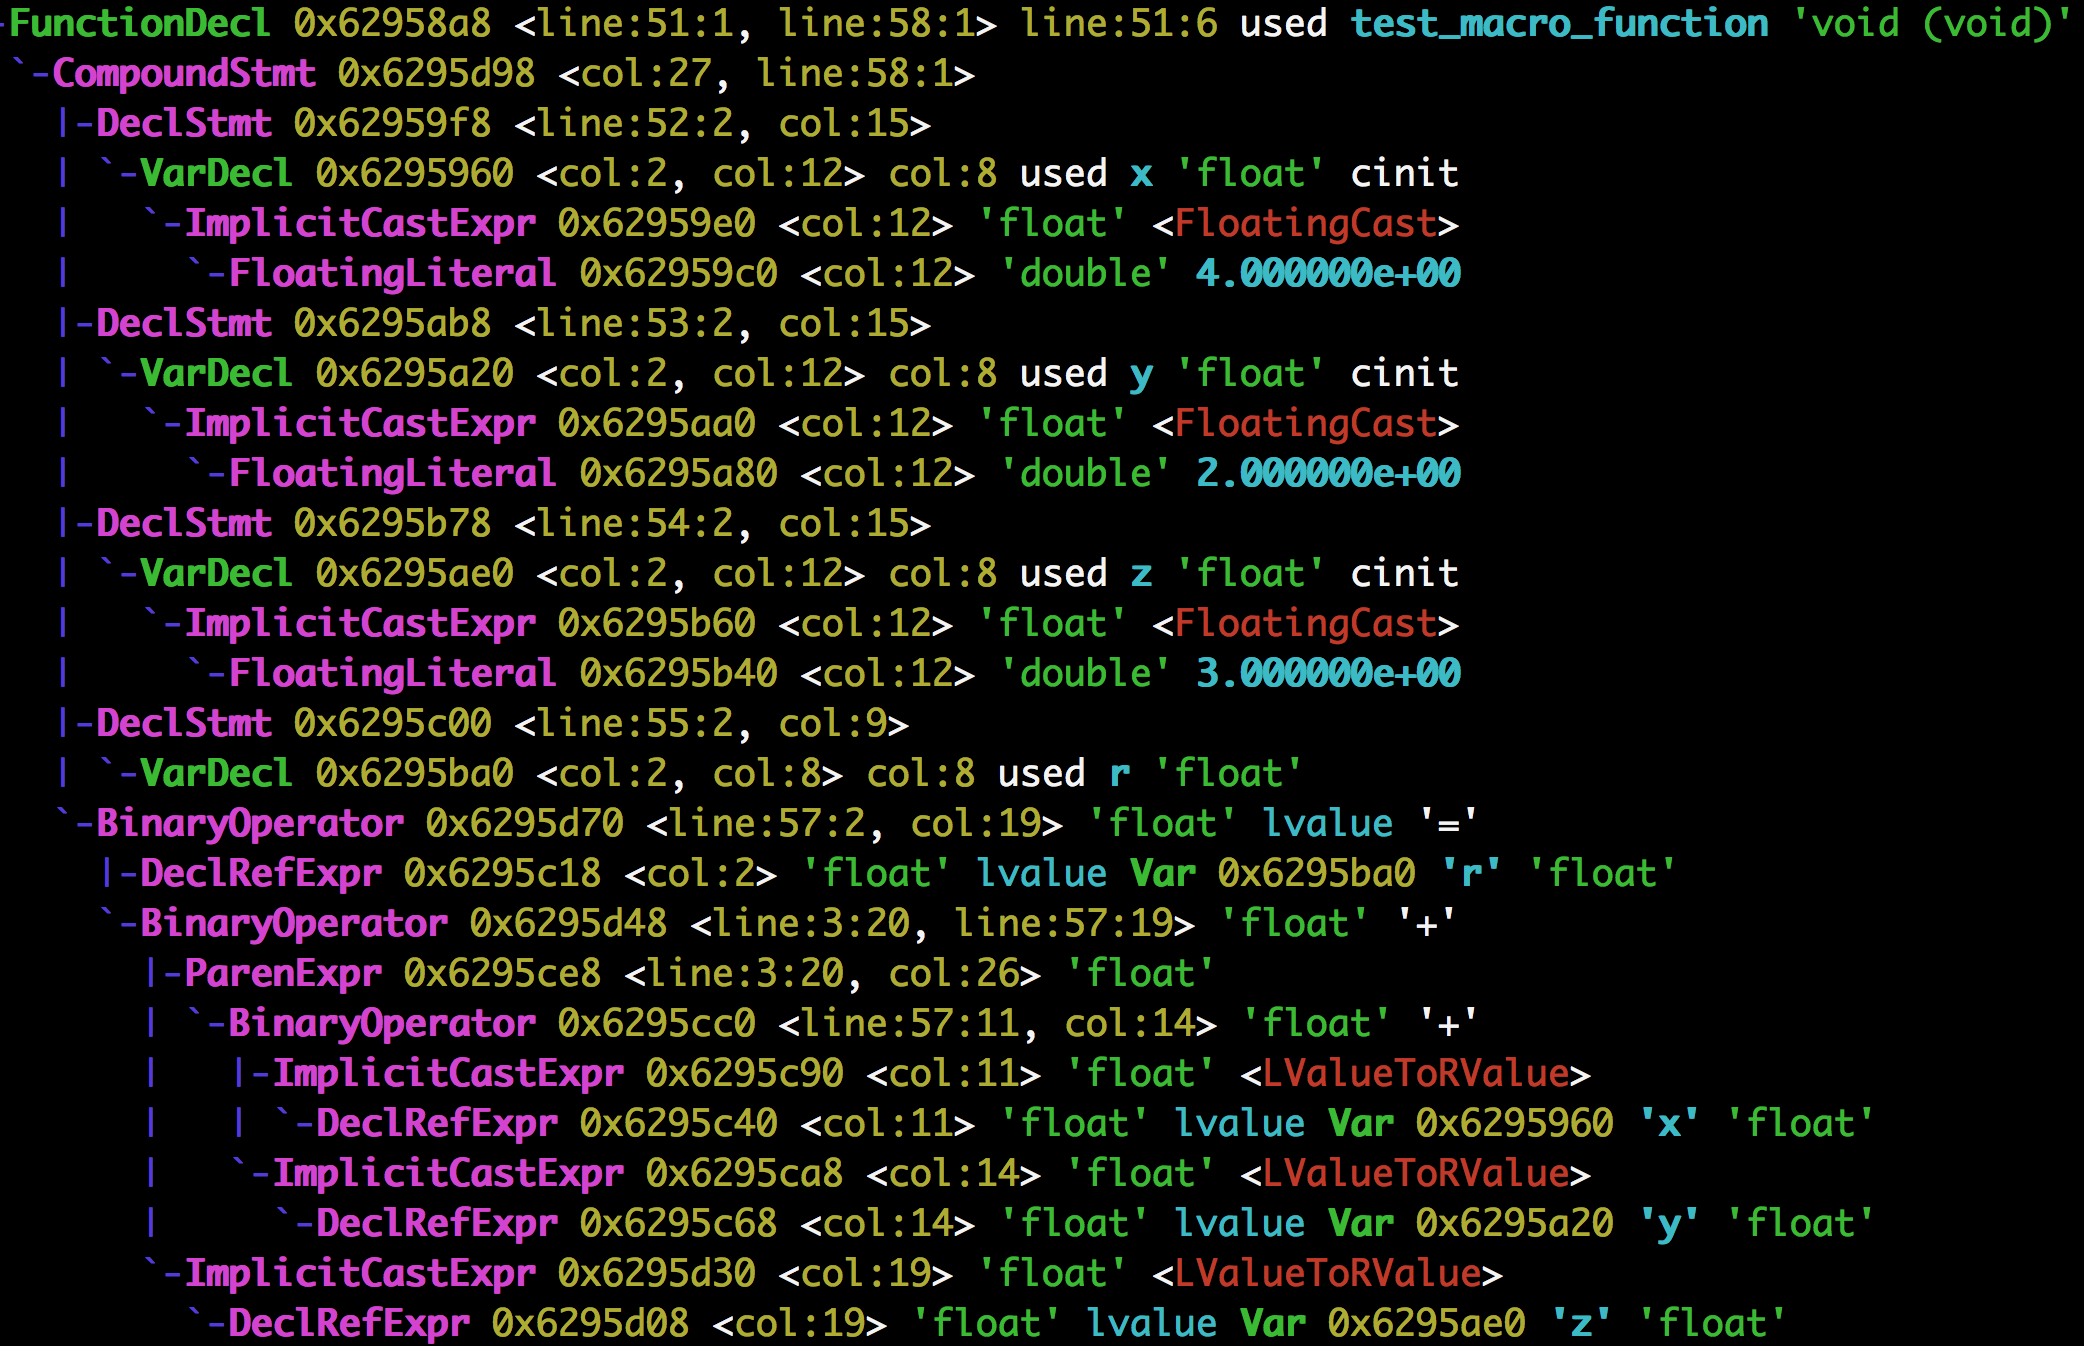
\includegraphics[width=15cm]{ast-sample.png}
\centering
\caption{Detecting Implicit Cast to decide the mutation process}
\end{figure}
This approach will ensure that even if the constructor does not have implemetation for the data type, everything will still work as expected. The result of the mutation after debugging for (\textit{2}) is as below
\begin{minted}[fontsize=\normalsize]{cpp}
	r = (float)(::vpa::VPA((float)k, OP_1)/::vpa::VPA((float)N, OP_1));
\end{minted}
Another way to deal with this problem is to modify the Approximate Operator library to have support for at least all basic data type. However, sometimes the intention is to only include an implentation for certain data type, depending on the purpose of the Approximate Operator. \\
~\\
The problem of (\textit{3}) and (\textit{4}) was a bit tricky to debug on account of the fact that some information returned by the AST is missing. In the case of (\textit{3}), as the macro is only a Literal Value, we follow the same principle as we did on the previous problem, performing check for appearances of \textit{Macro} and \textit{Literal} statement classes, then perform mutation accordingly. The same, however, can not be applied to (\textit{4}) because this is a function-like Macro with arguments which made debugging dfficult, espcially when the information returned from the Abstract Syntax Tree is missing. Currently, we do not have any solution for this problem so we try to avoid using projects or parts of the project that contains this kind of Pre-processor. The best we can do is to try and replace these function-like Macros with proper functions. \\
~\\
The debugged version of Chimera can be found at: \url{https://github.com/nnkhoa/clang-chimera}\\
\section{Compatibility with Artificial Neural Network libraries}

\subsection{Darknet}
Placeholder
\subsection{Fast Artificial Neural Network(FANN)}
Placeholder